\documentclass[12pt]{article}
\usepackage[utf8]{inputenc}
\usepackage{microtype}
\usepackage{graphicx}
% \usepackage{subfigure}
\usepackage{booktabs} % for professional tables
\usepackage{hyperref}
\usepackage{amsmath}
\usepackage{amssymb}
\usepackage{mathtools}
\usepackage{amsthm}
\usepackage{footnote}
\usepackage{mathtools}
\usepackage[flushleft]{threeparttable}
\usepackage{etoolbox}
\usepackage{nicefrac}       % compact symbols for 1/2, etc.
\usepackage{microtype}      % microtypography
\usepackage{xcolor}         % colors
\usepackage{enumitem}
\usepackage{tabularx}
\usepackage[margin=0.5in]{geometry}


%\usepackage{charter}
%\usepackage{calc}

\usepackage{multirow}
% \usepackage[cp1250]{inputenc}
% \usepackage[T1]{fontenc}
% \usepackage{calligra}
\usepackage{layout}

% AMS
\usepackage{amsmath}
\usepackage{amsthm}
\usepackage{amssymb}
\usepackage{amsfonts}
\usepackage{mathtools}
\usepackage{siunitx}

\usepackage{bbm}

\usepackage{url}
\usepackage{color}
\usepackage{graphicx}
\usepackage{algorithmic}
\usepackage{algorithm}
\usepackage{verbatim}

\usepackage{apptools}
\usepackage{thmtools}
% \usepackage{algpseudocode}

% paper specific macros
\newcommand{\g}{{\color{red}g}}
\newcommand{\h}{{\color{blue}h}}

% general macros

\newcommand{\norm}[1]{\left\| #1 \right\|}
\newcommand{\sqnorm}[1]{\left\| #1 \right\|^2}
\newcommand{\lin}[1]{\left\langle #1\right\rangle} % inner product
\newcommand{\inp}[2]{\left\langle#1,#2\right\rangle} % inner product

% caligraphic
\newcommand{\cA}{\mathcal{A}}
\newcommand{\cB}{\mathcal{B}}
\newcommand{\cC}{\mathcal{C}}
\newcommand{\cD}{\mathcal{D}}
\newcommand{\cH}{\mathcal{H}}
\newcommand{\cL}{\mathcal{L}}
\newcommand{\cO}{\mathcal{O}}
\newcommand{\cQ}{\mathcal{Q}}
\newcommand{\cS}{\mathcal{S}}
\newcommand{\cW}{\mathcal{W}}
\newcommand{\cY}{\mathcal{Y}}
\newcommand{\cZ}{\mathcal{Z}}

% bold matrices
\newcommand{\mM}{\mathbf{M}}
\newcommand{\mN}{\mathbf{N}}
\newcommand{\mI}{\mathbf{I}}
\newcommand{\mJ}{\mathbf{J}}
\newcommand{\mL}{\mathbf{L}}
\newcommand{\mD}{\mathbf{D}}
\newcommand{\mO}{\mathbf{O}}


% strange stuff
\newcommand{\hotidea}{{\color{red}\bf HOT IDEA: }}
\newcommand{\done}{{\color{blue}\bf DONE: }}
\newcommand{\del}[1]{}
\let\la=\langle
\let\ra=\rangle

% basic macros
\newcommand{\R}{\mathbb{R}} % reals
\newcommand{\U}{\mathbb{U}} % reals
\newcommand{\PermComp}{\U\mathbb{P}} % reals

\newcommand{\st}{\;:\;} % such that
%\newcommand{\eqdef}{\stackrel{\text{def}}{=}}
\newcommand{\eqdef}{:=} %\vcentcolon

\newcommand{\Prob}{\mathbf{Prob}} % probability
\newcommand{\ProbCond}[2]{\Prob\left(\left.#1\right\vert#2\right)}

\newcommand{\nnz}[1]{{\color{red}\|#1\|_0}}

% sets
\DeclareMathOperator{\card}{card}         % cardinality of a set
\DeclareMathOperator{\diam}{diam}        % diameter of a set
\DeclareMathOperator{\vol}{vol}               % volume of a set

% statistics
\newcommand{\Exp}[1]{{\rm E}\left[#1\right]}
\newcommand{\ExpCond}[2]{{\rm E}\left[\left.#1\right\vert#2\right]}
\newcommand{\ExpSub}[2]{{\rm E}_{#1}\left[#2\right]}
\DeclareMathOperator{\Cov}{Cov}         % covariance
\DeclareMathOperator{\Var}{Var}         % variance
\DeclareMathOperator{\Corr}{Corr}       % correlation

% functions and operators
\DeclareMathOperator{\signum}{sign}     % signum/sign of a scalar
\DeclareMathOperator{\dom}{dom}         % domain
\DeclareMathOperator{\epi}{epi}         % epigraph
\DeclareMathOperator{\Ker}{null}        % nullspace/kernel
\DeclareMathOperator{\nullspace}{null}  % nullpsace
\DeclareMathOperator{\range}{range}     % range
\DeclareMathOperator{\Image}{Im}        % image

% topology
\DeclareMathOperator{\interior}{int}    % interior
\DeclareMathOperator{\ri}{rint}         % relative interior
\DeclareMathOperator{\rint}{rint}       % relative interior
\DeclareMathOperator{\bdry}{bdry}       % boundary
\DeclareMathOperator{\cl}{cl}           % closure

% vectors, matrices
\DeclareMathOperator{\linspan}{span}
\DeclareMathOperator{\linspace}{linspace}
\DeclareMathOperator{\cone}{cone}

\DeclareMathOperator{\tr}{tr}           % trace
\DeclareMathOperator{\rank}{rank}       % rank
\DeclareMathOperator{\conv}{conv}       % convex hull
\DeclareMathOperator{\Diag}{Diag}       % Diag(v) = diagonal matrix with v_i on the diagonal
\DeclareMathOperator{\diag}{diag}       % diag(D) = the diagonal vector of matrix D
\DeclareMathOperator{\Arg}{Arg}         % Argument

%\renewcommand{\qedsymbol}{\ding{114}}




%%%%%%%%

% TODO: Fix here fonts
\newcommand{\Sample}{\mathcal{S}}
%\newcommand{\E}{\mathbb{E}}
%\newcommand{\norm}[1]{\left\lVert#1\right\rVert_2}
\newcommand{\B}{\mathbb{B}}


\usepackage{tcolorbox}
\usepackage{pifont}
\definecolor{mydarkgreen}{RGB}{39,130,67}
\definecolor{mydarkred}{RGB}{192,47,25}
\newcommand{\green}{\color{mydarkgreen}}
\newcommand{\red}{\color{mydarkred}}
\newcommand{\cmark}{\green\ding{51}}%
\newcommand{\xmark}{\red\ding{55}}%

\newcommand{\algname}[1]{{\green\small \sf #1}}
\newcommand{\algnamesmall}[1]{{\green\scriptsize \sf #1}}

\newcommand{\tablescriptsize}[1]{{\scriptsize #1}}
\newcommand{\tablesmall}[1]{{\small #1}}



%%%%%%%%

\newtheorem{assumption}{Assumption}
\newtheorem{lemma}{Lemma}
\newtheorem{algorithms}{Algorithm}
\newtheorem{theorem}{Theorem}
\newtheorem{proposition}{Proposition}
\newtheorem{example}{Example}
\newtheorem{corollary}{Corollary}

\theoremstyle{plain}

\newtheorem{prop}[theorem]{Proposition}
\newtheorem{cor}[theorem]{Corollary}
\newtheorem{lem}[theorem]{Lemma}
\newtheorem{claim}[theorem]{Claim}
\newtheorem{remark}[theorem]{Remark}

\theoremstyle{definition}

\newtheorem{exercise}[theorem]{Exercise}

\newtheorem{rem}[theorem]{Remark}
\newtheorem{que}[theorem]{Question}
\newtheorem{definition}[theorem]{Definition}

% Hack that enables labeling of lines in algorithms
\newcommand{\alglinelabel}{%
  \addtocounter{ALC@line}{-1}% Reduce line counter by 1
  \refstepcounter{ALC@line}% Increment line counter with reference capability
  \label% Regular \label
}

\begin{document}
\begin{center}
    Extra Experiments
\end{center}

In this experiments, we compare our new algorithm \algname{DASHA-PP} with previous baselines \algname{MARINA} and \algname{FRECON} in the partial participation setting. We consider \algname{MARINA} and \algname{FRECON} because they are the previous SOTA methods in the \emph{partial participation setting with compression}. We consider the same optimization problem and setup as in Section~A of the paper.
% \section*{Warm Up: Gradient Setting}
% \begin{figure}[h]
% 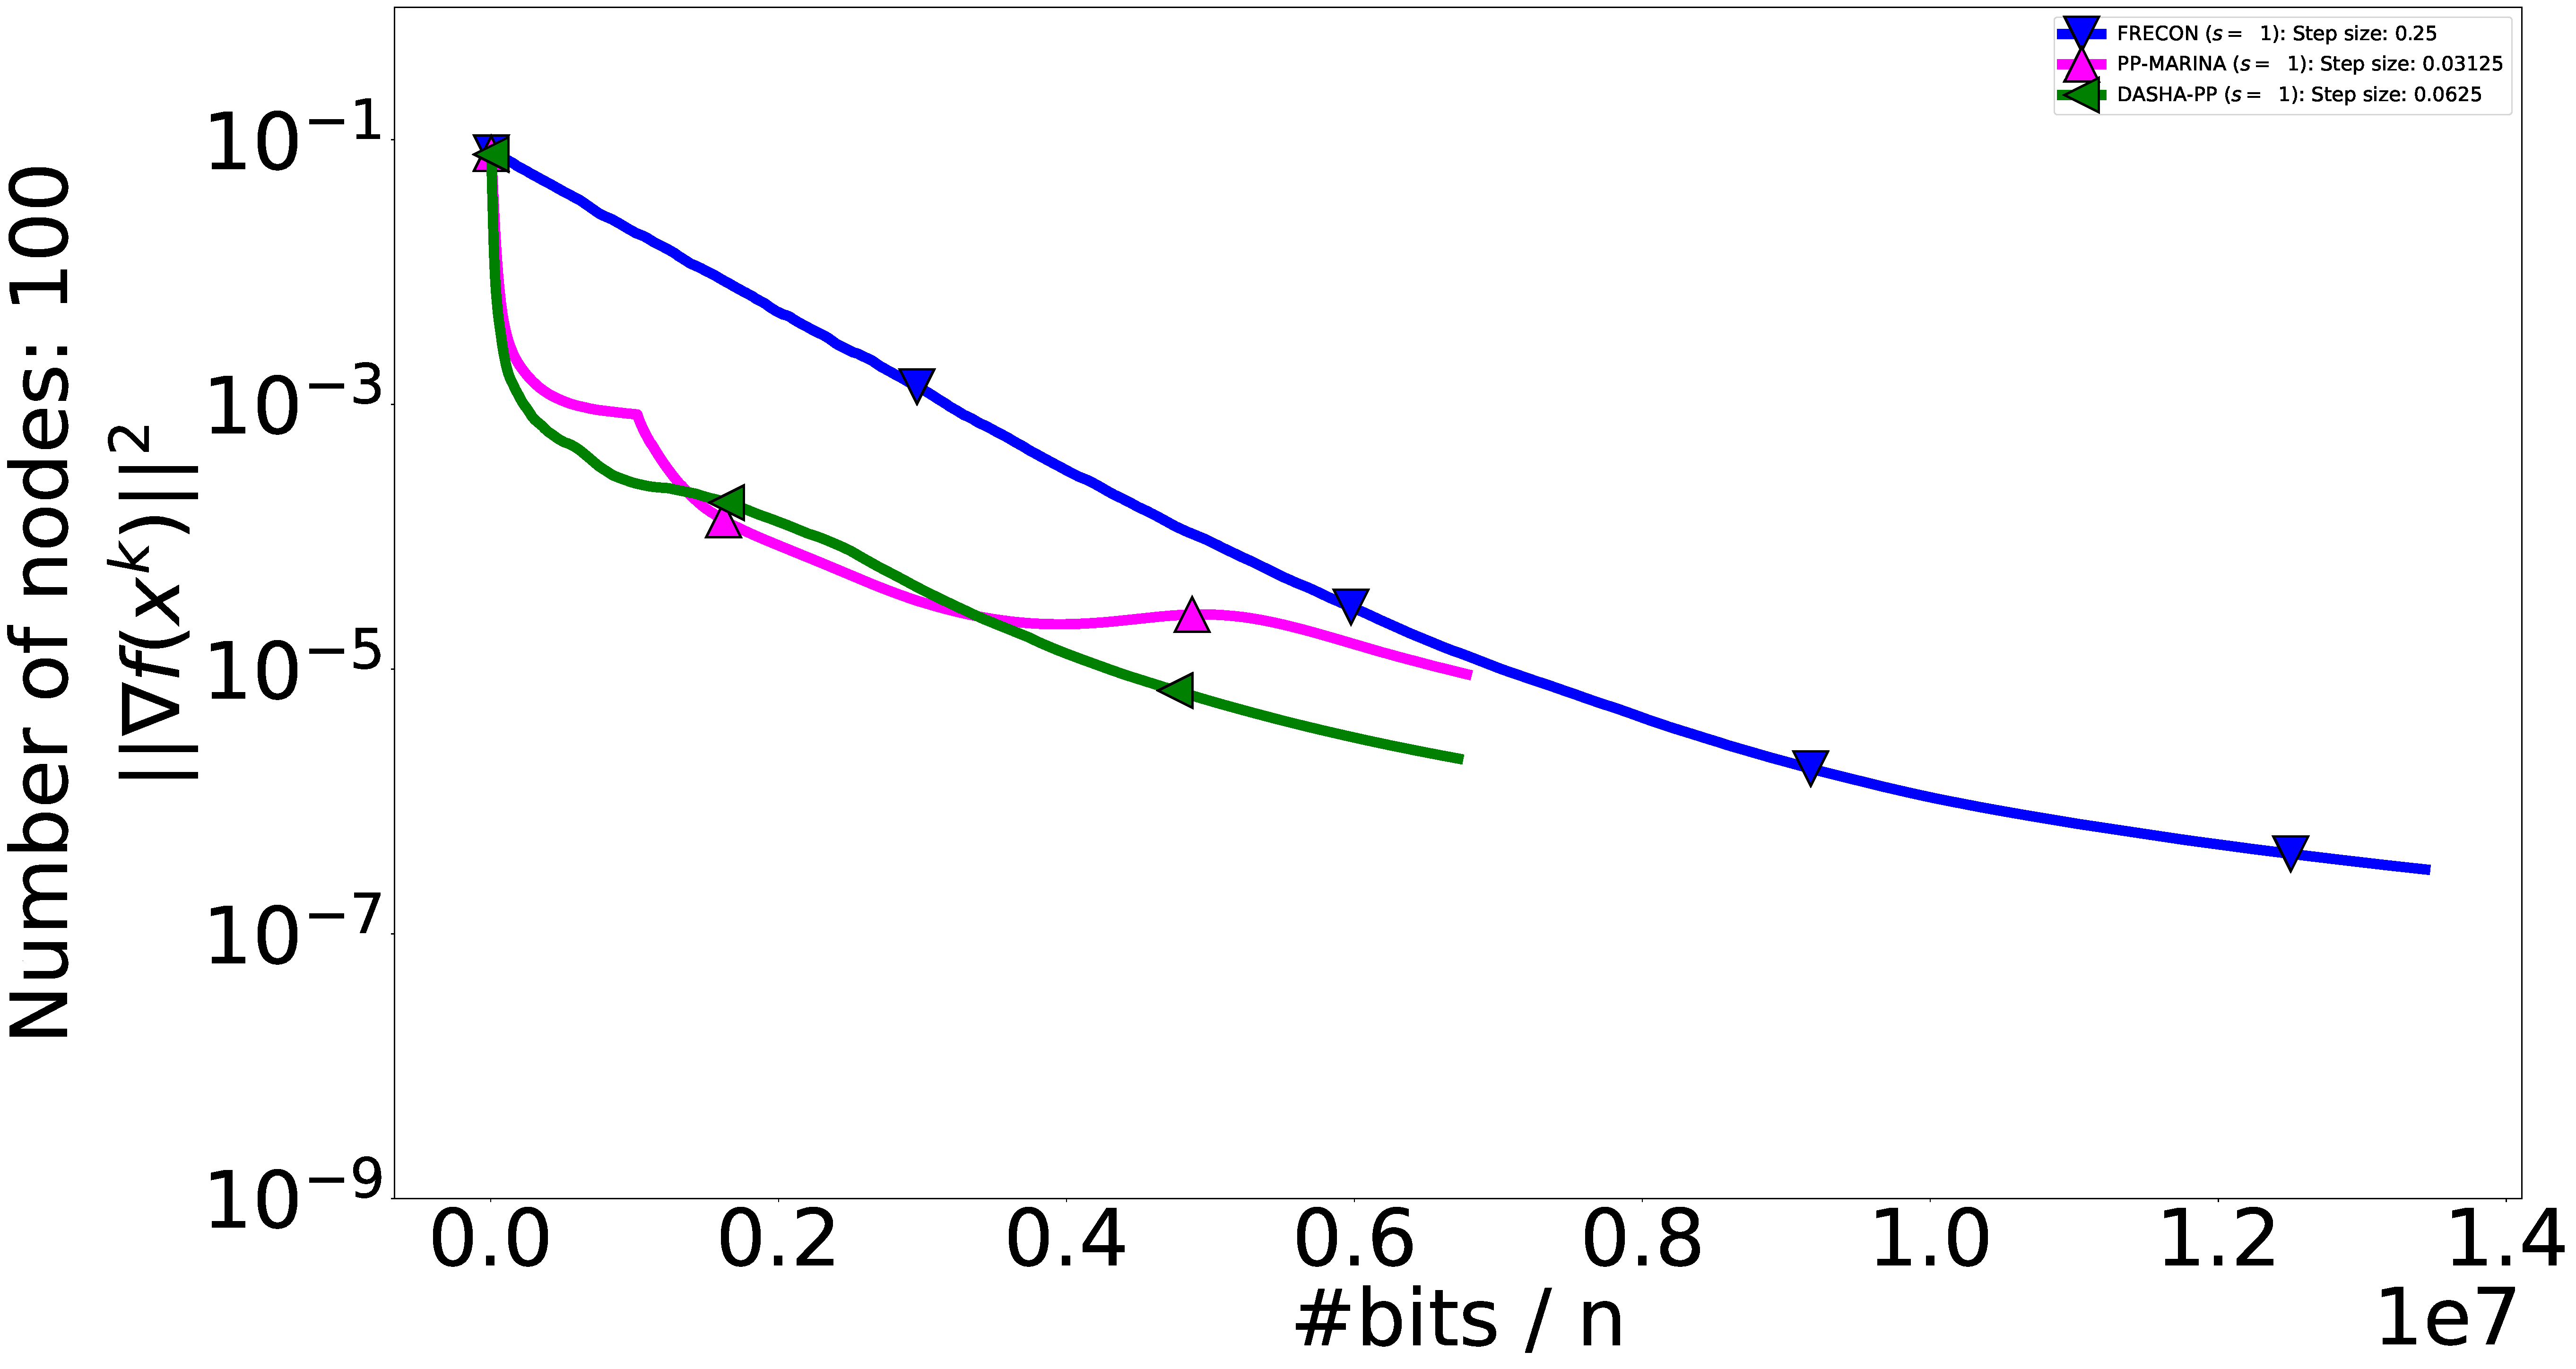
\includegraphics[width=\textwidth]{neurips_2022_gradient_mushrooms_nodes_100_coord_10_prob_0_01_seeds_3_no_init_with_pp_marina.pdf}
% \caption{Classification task with the \textit{mushrooms} dataset.}
% \label{fig:gradient}
% \end{figure}

\begin{center}
    \bf Stochastic Setting
\end{center}

In Figure~\ref{fig:stochastic}, we compare all three methods in the stochastic setting on two different datasets: \textit{real-sim} and \textit{MNIST}. The parameter $s$ means the number of clients participating in each round. We can see that \algname{DASHA-PP} has better convergence rates than \algname{FRECON}. \algname{DASHA-PP} with $s \in \{5, 10\}$ even improves \algname{MARINA} that works in the full participation regime (one should expect that convergence rate of \algname{MARINA} with partial participation will be even worse).

\begin{figure}[H]
    \begin{subfigure}{.5\textwidth}
        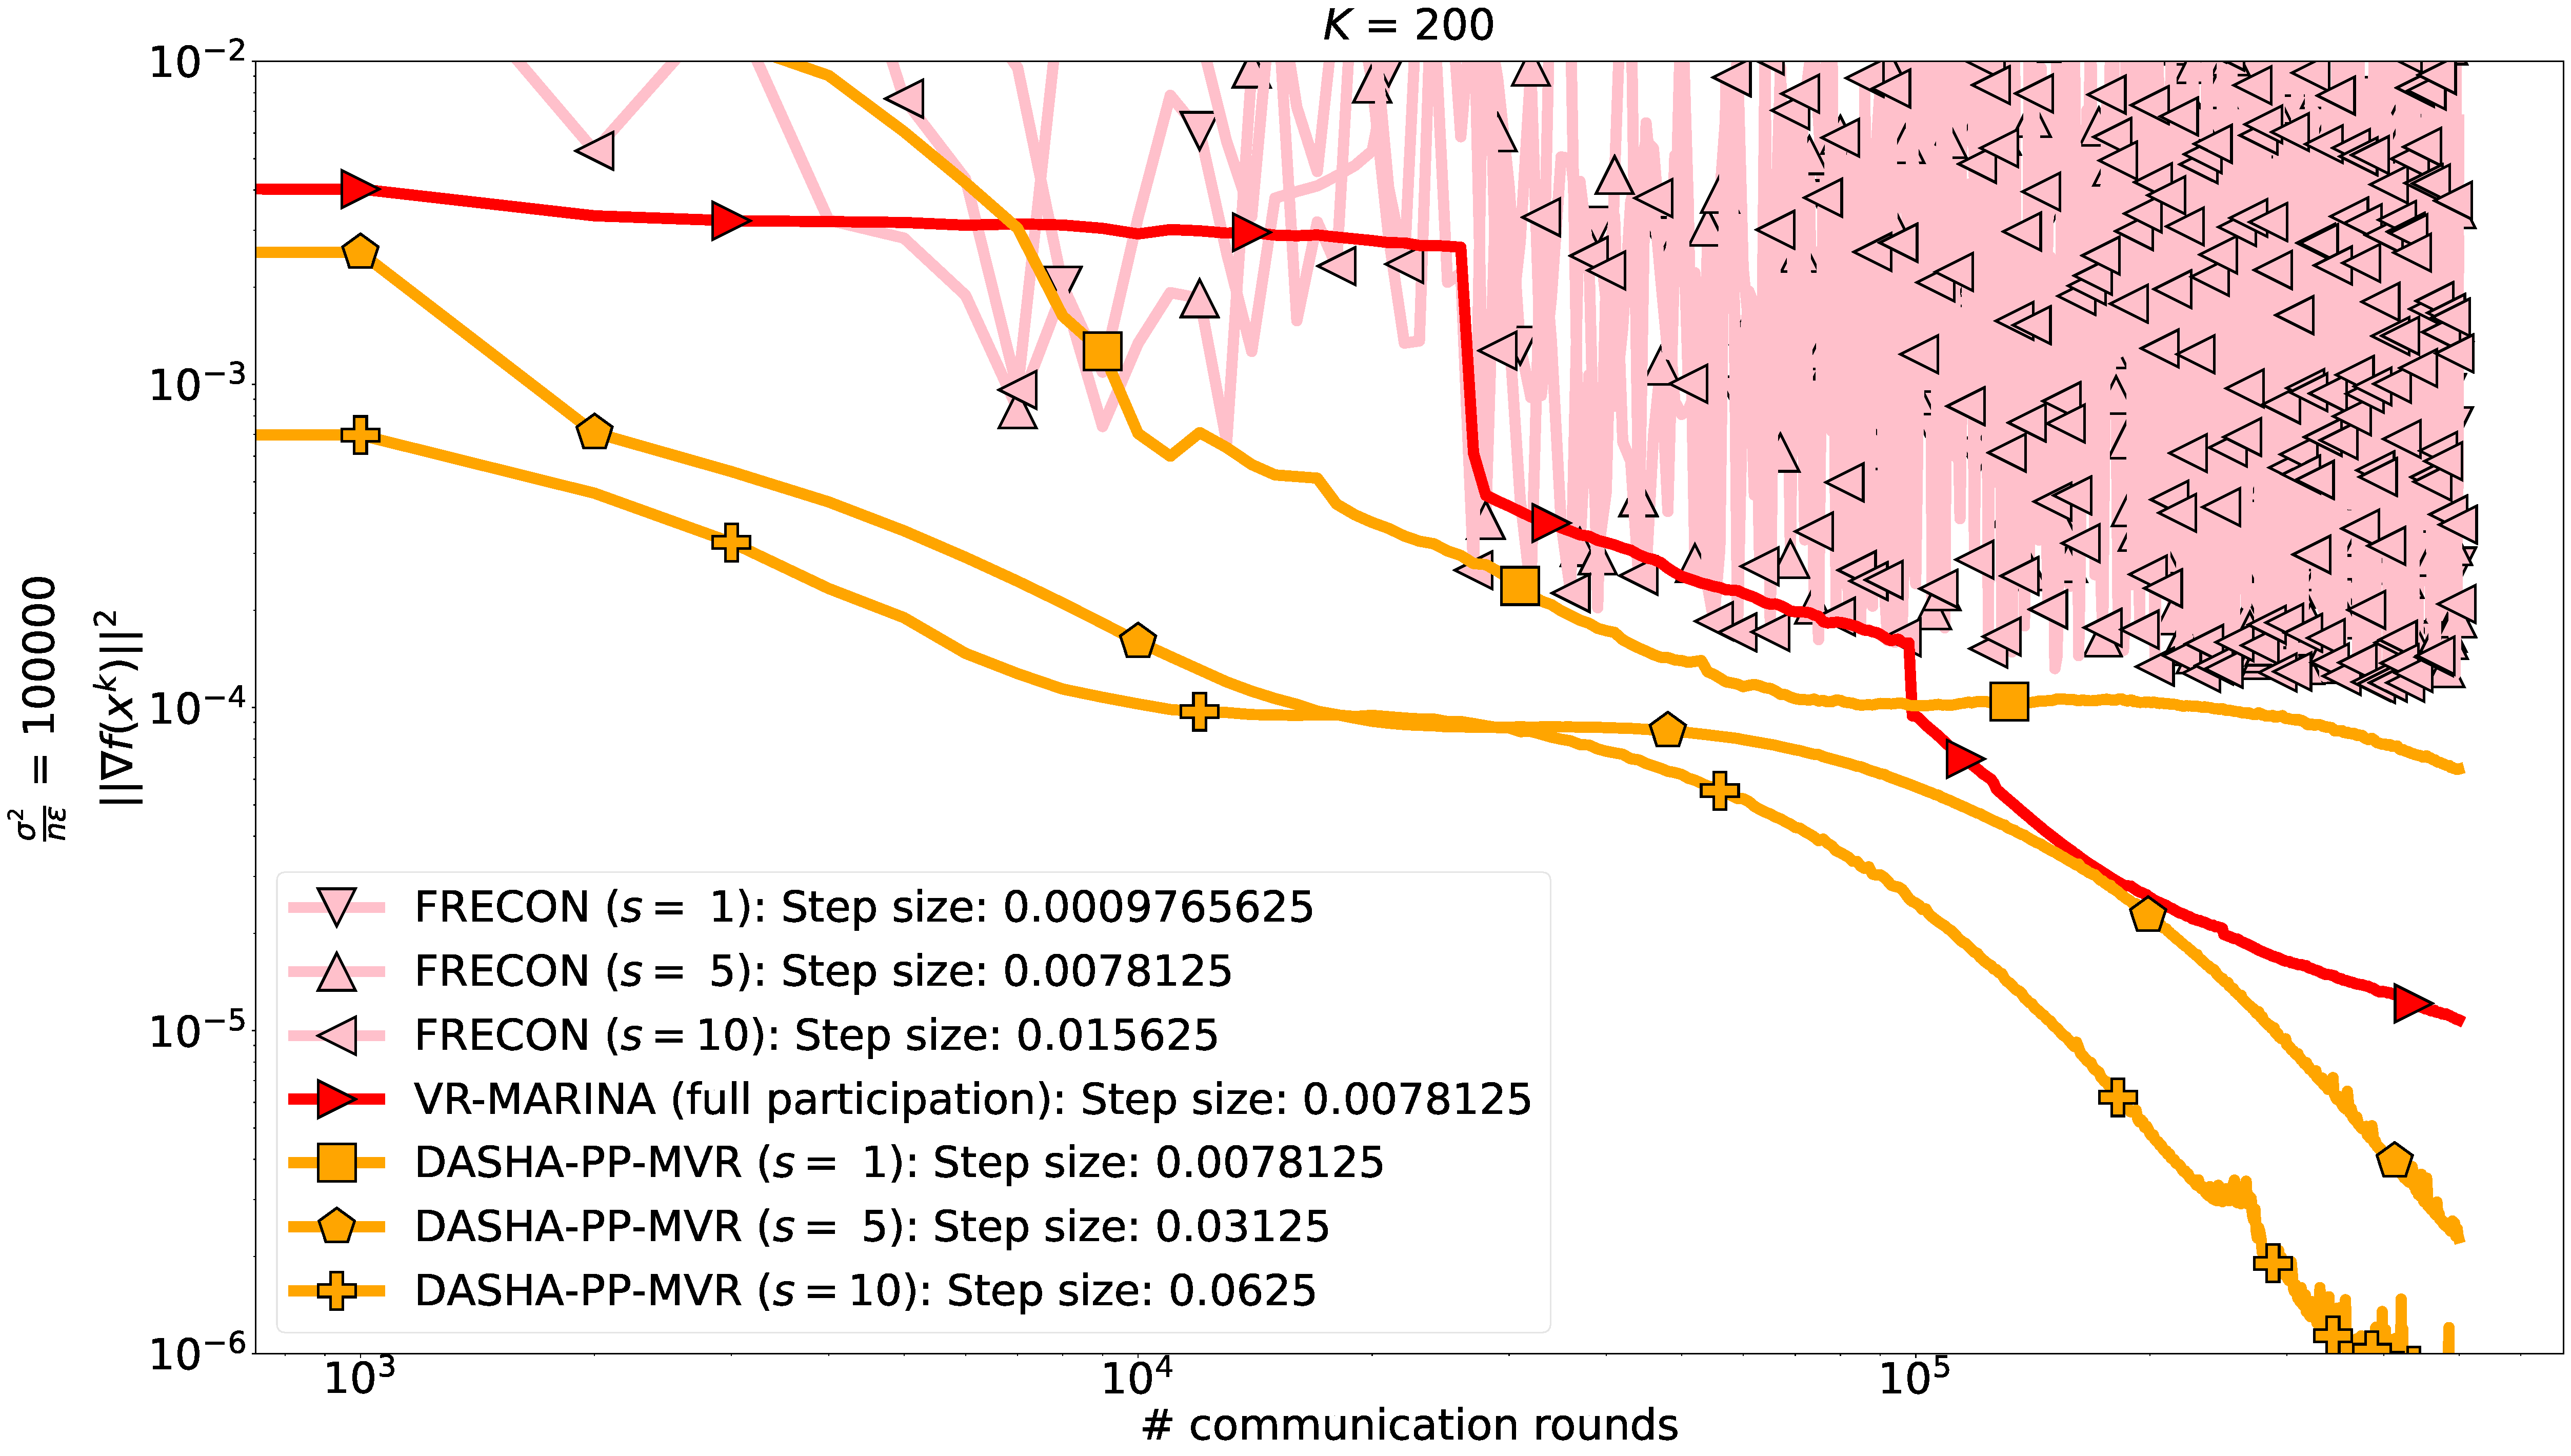
\includegraphics[width=\textwidth]{neurips_2022_stochastic_real-sim_nof_200_numnodes_10_probs_mega_batch_100000_fix_nm_bug.pdf}
        \caption{\textit{real-sim}}
    \end{subfigure}
    \begin{subfigure}{.5\textwidth}
        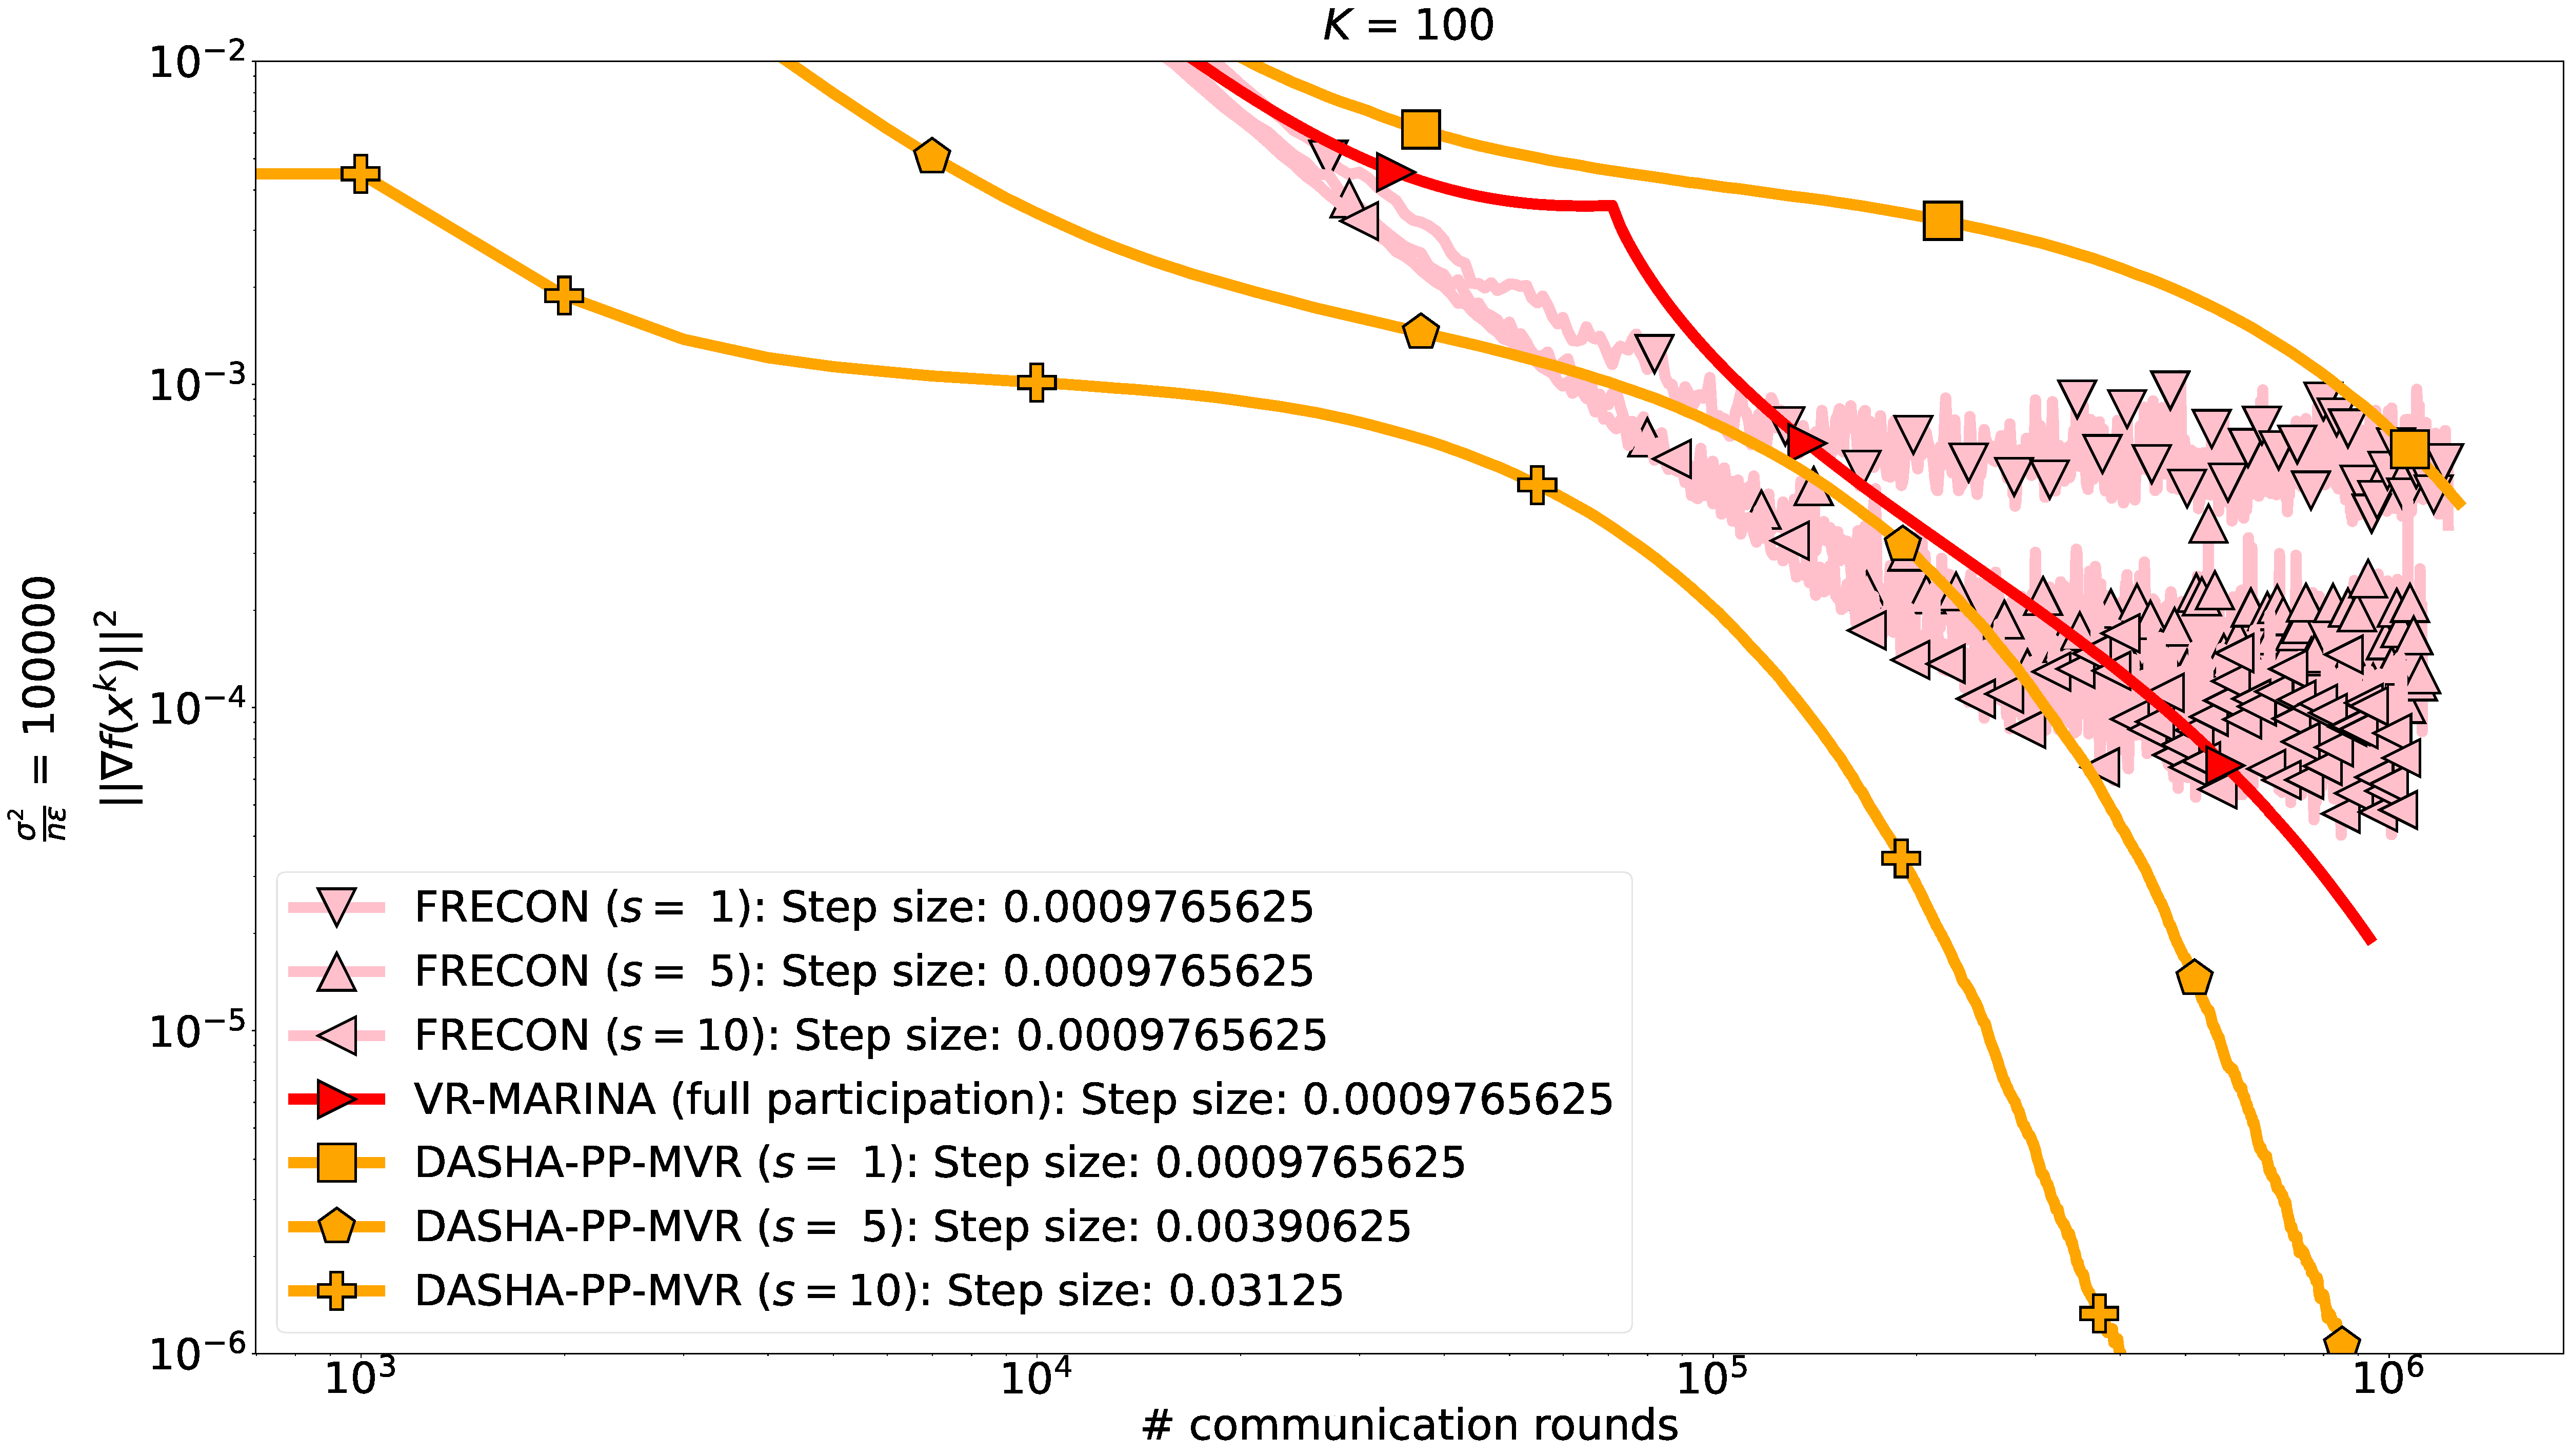
\includegraphics[width=\textwidth]{neurips_2023_stochastic_mnist_nof_100_numnodes_10_probs_mega_batch_100000_batch_size_10_longer.pdf}
        \caption{\textit{MNIST}}
    \end{subfigure}
\caption{Classification task with the \textit{mushrooms} dataset.}
\label{fig:stochastic}
\end{figure}

\begin{center}
    \bf Finite-Sum Setting
\end{center}
In Figure~\ref{fig:finite-sum}, we consider the finite-sum setting. We do not have experiments with \algname{FRECON} because the authors of \algname{FRECON} do not consider it in the finite-sum setting. We can see that \algname{DASHA-PP} with $s \in \{50, 90, 100\}$ converges faster than \algname{MARINA} (that works in the full participation regime).

\begin{figure}[H]
    \begin{subfigure}{.5\textwidth}
        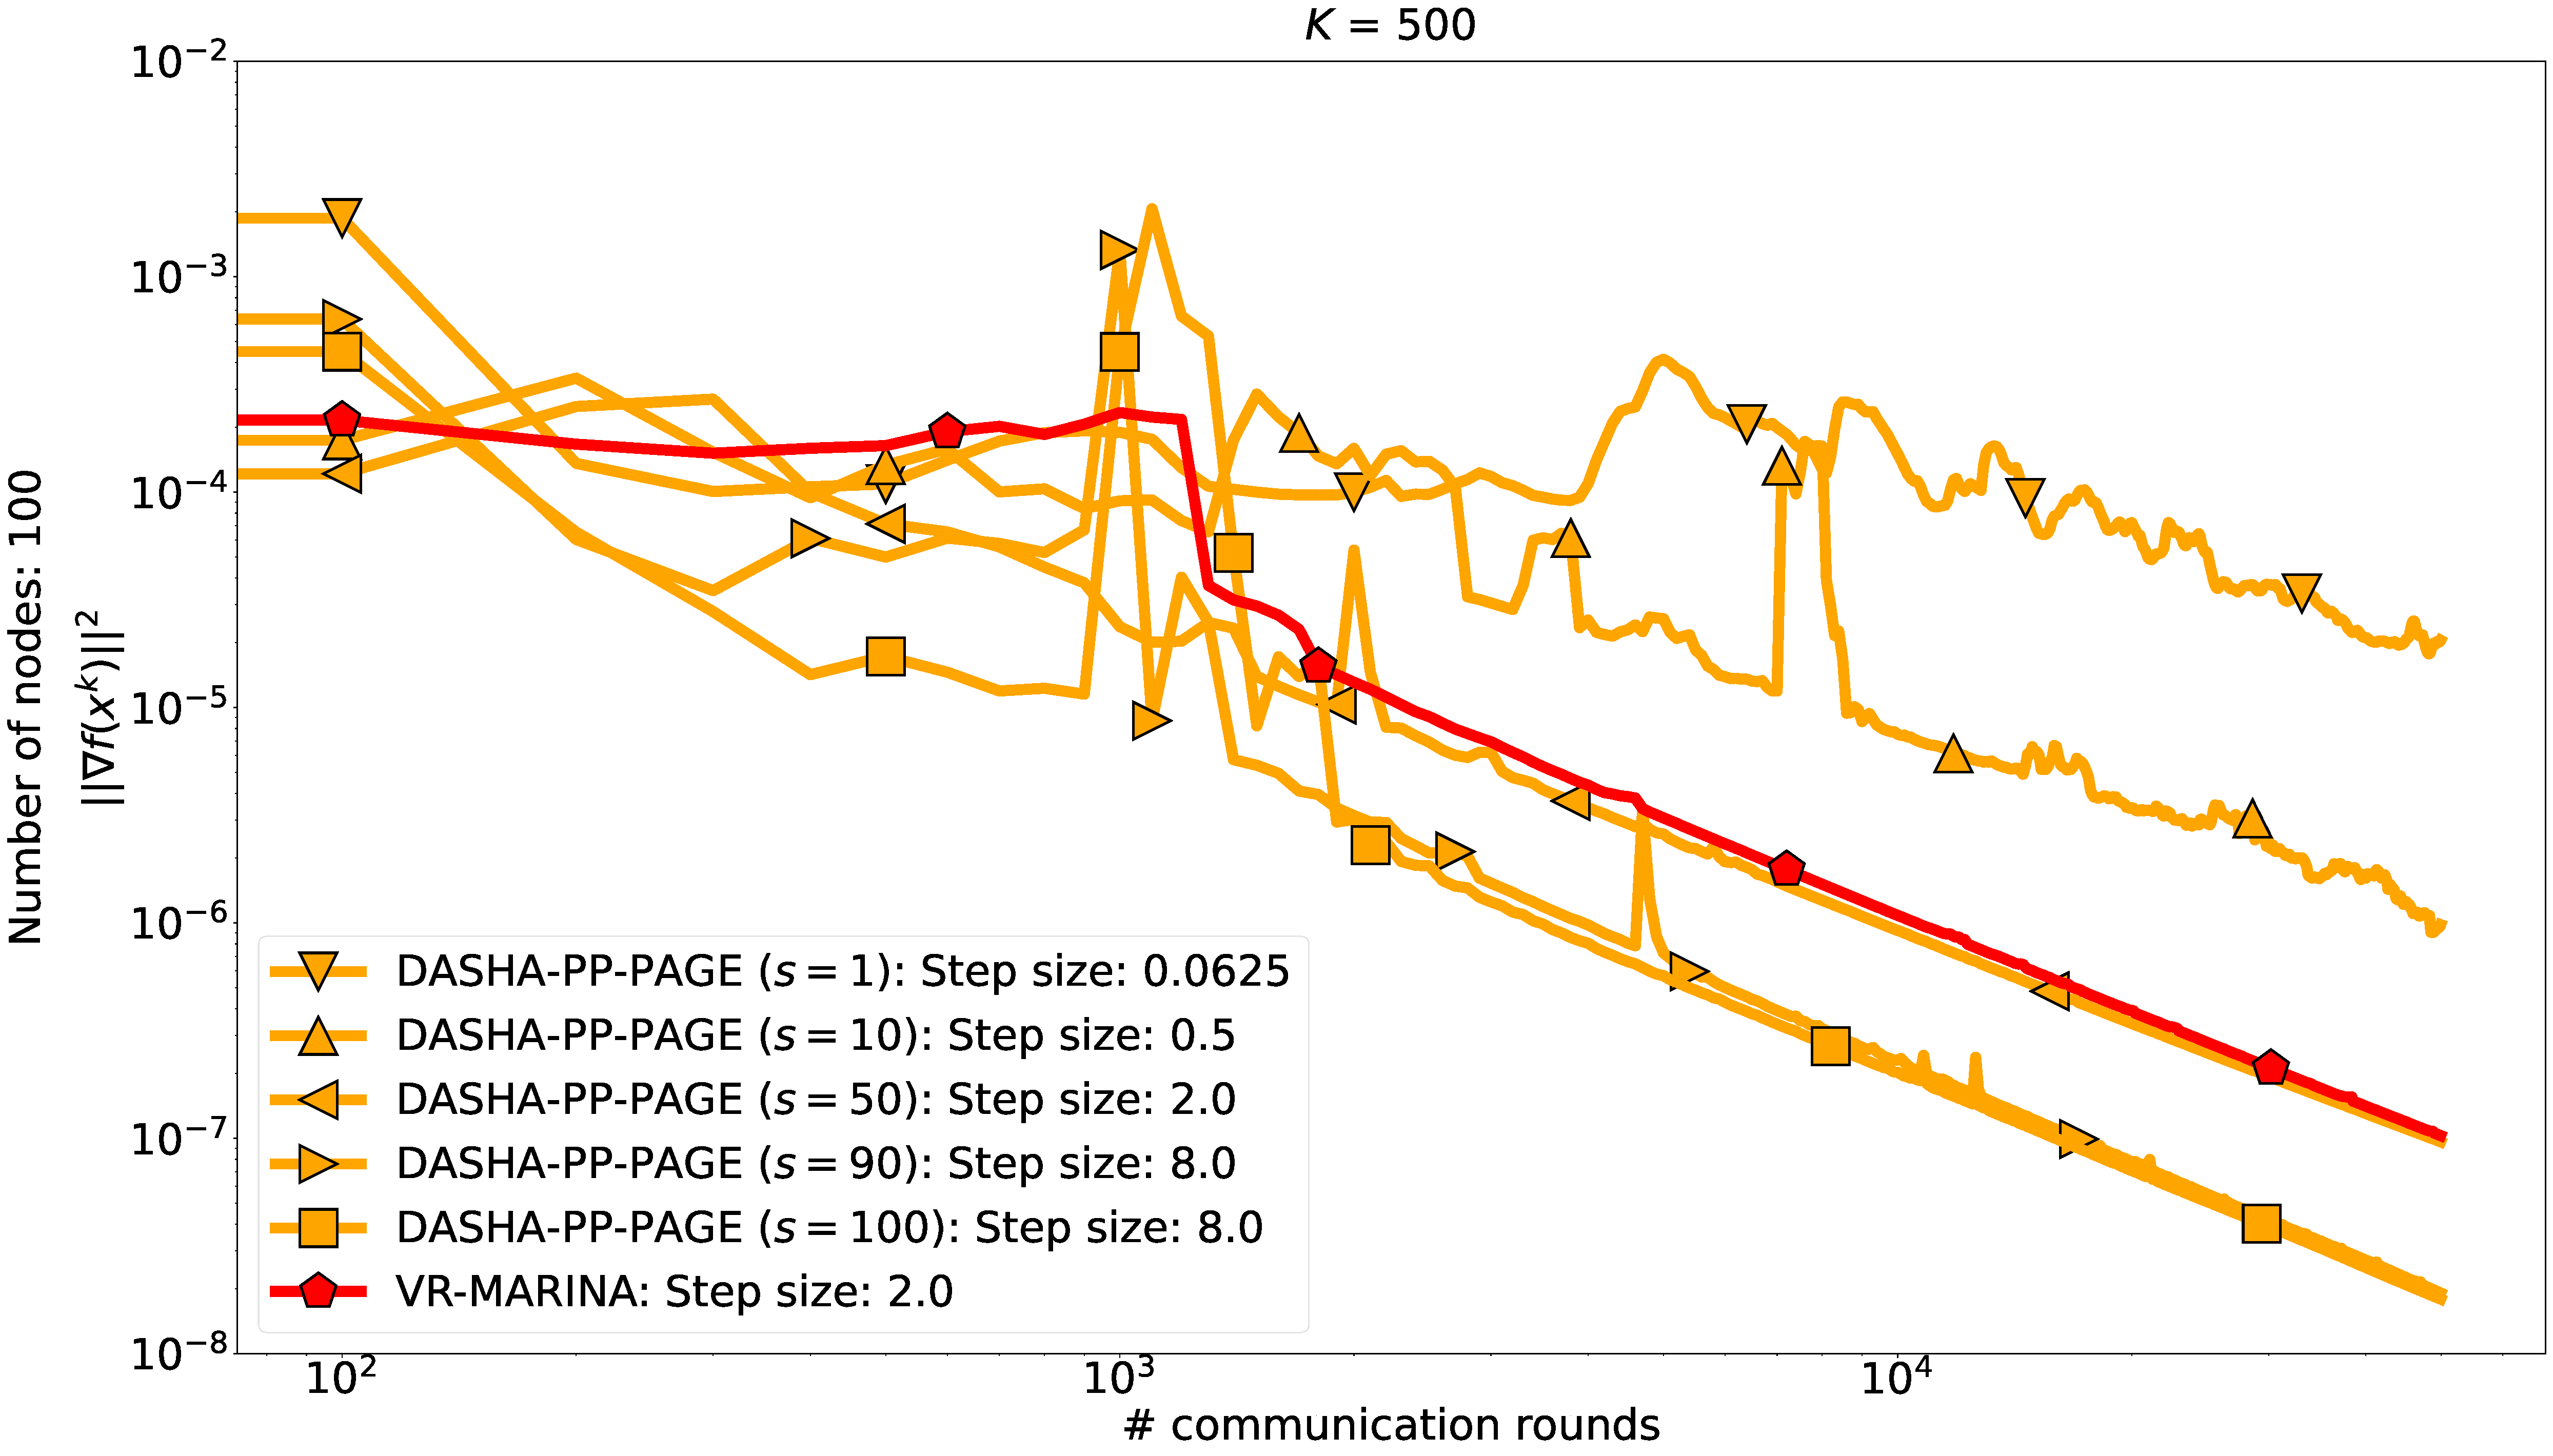
\includegraphics[width=\textwidth]{neurips_2022_finite_sum_real-sim_nof_500_numnodes_100_more_probs_batch_size_1.pdf}
        \caption{MNIST, BZ = 10}
    \end{subfigure}
    \begin{subfigure}{.5\textwidth}
        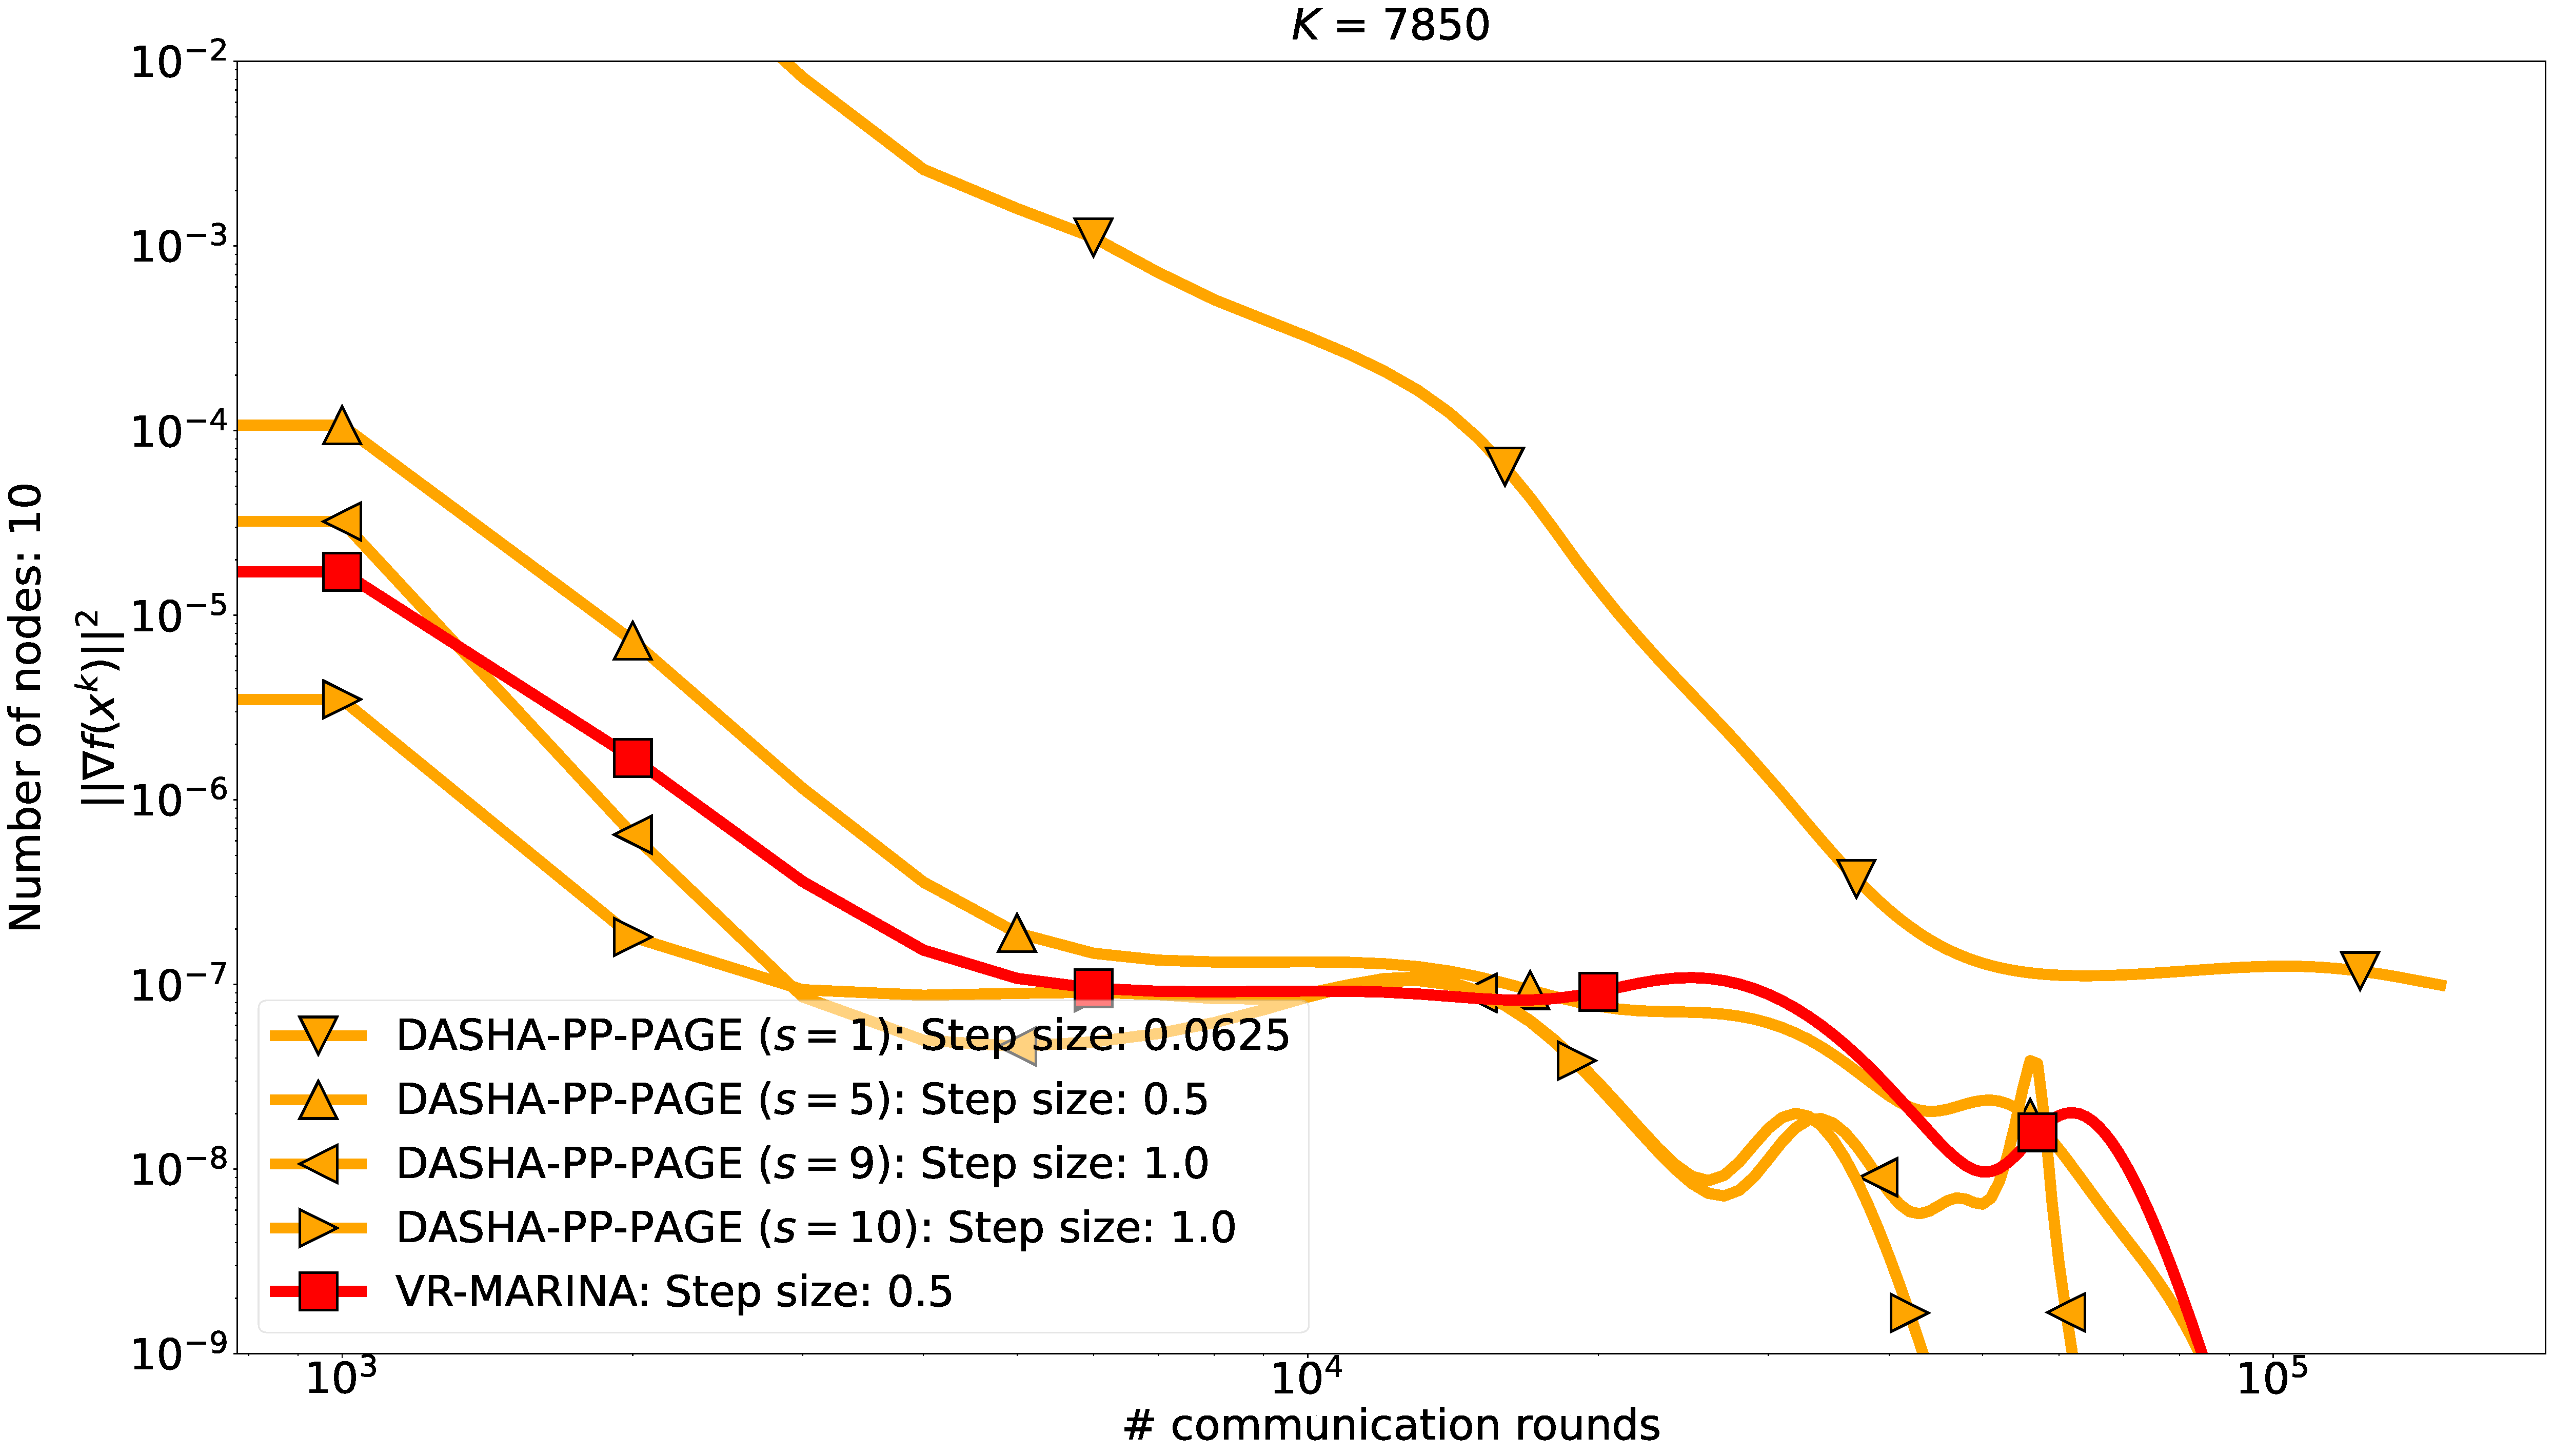
\includegraphics[width=\textwidth]{neurips_2022_finite_sum_mnist_nof_7850_numnodes_10_more_probs_batch_size_100_split_by_labels_logistic.pdf}
        \caption{MNIST, BZ = 100}
    \end{subfigure}
\caption{Classification task with the \textit{mushrooms} dataset.}
\label{fig:finite-sum}
\end{figure}

% \begin{figure}[H]
%     \begin{subfigure}{.5\textwidth}
%         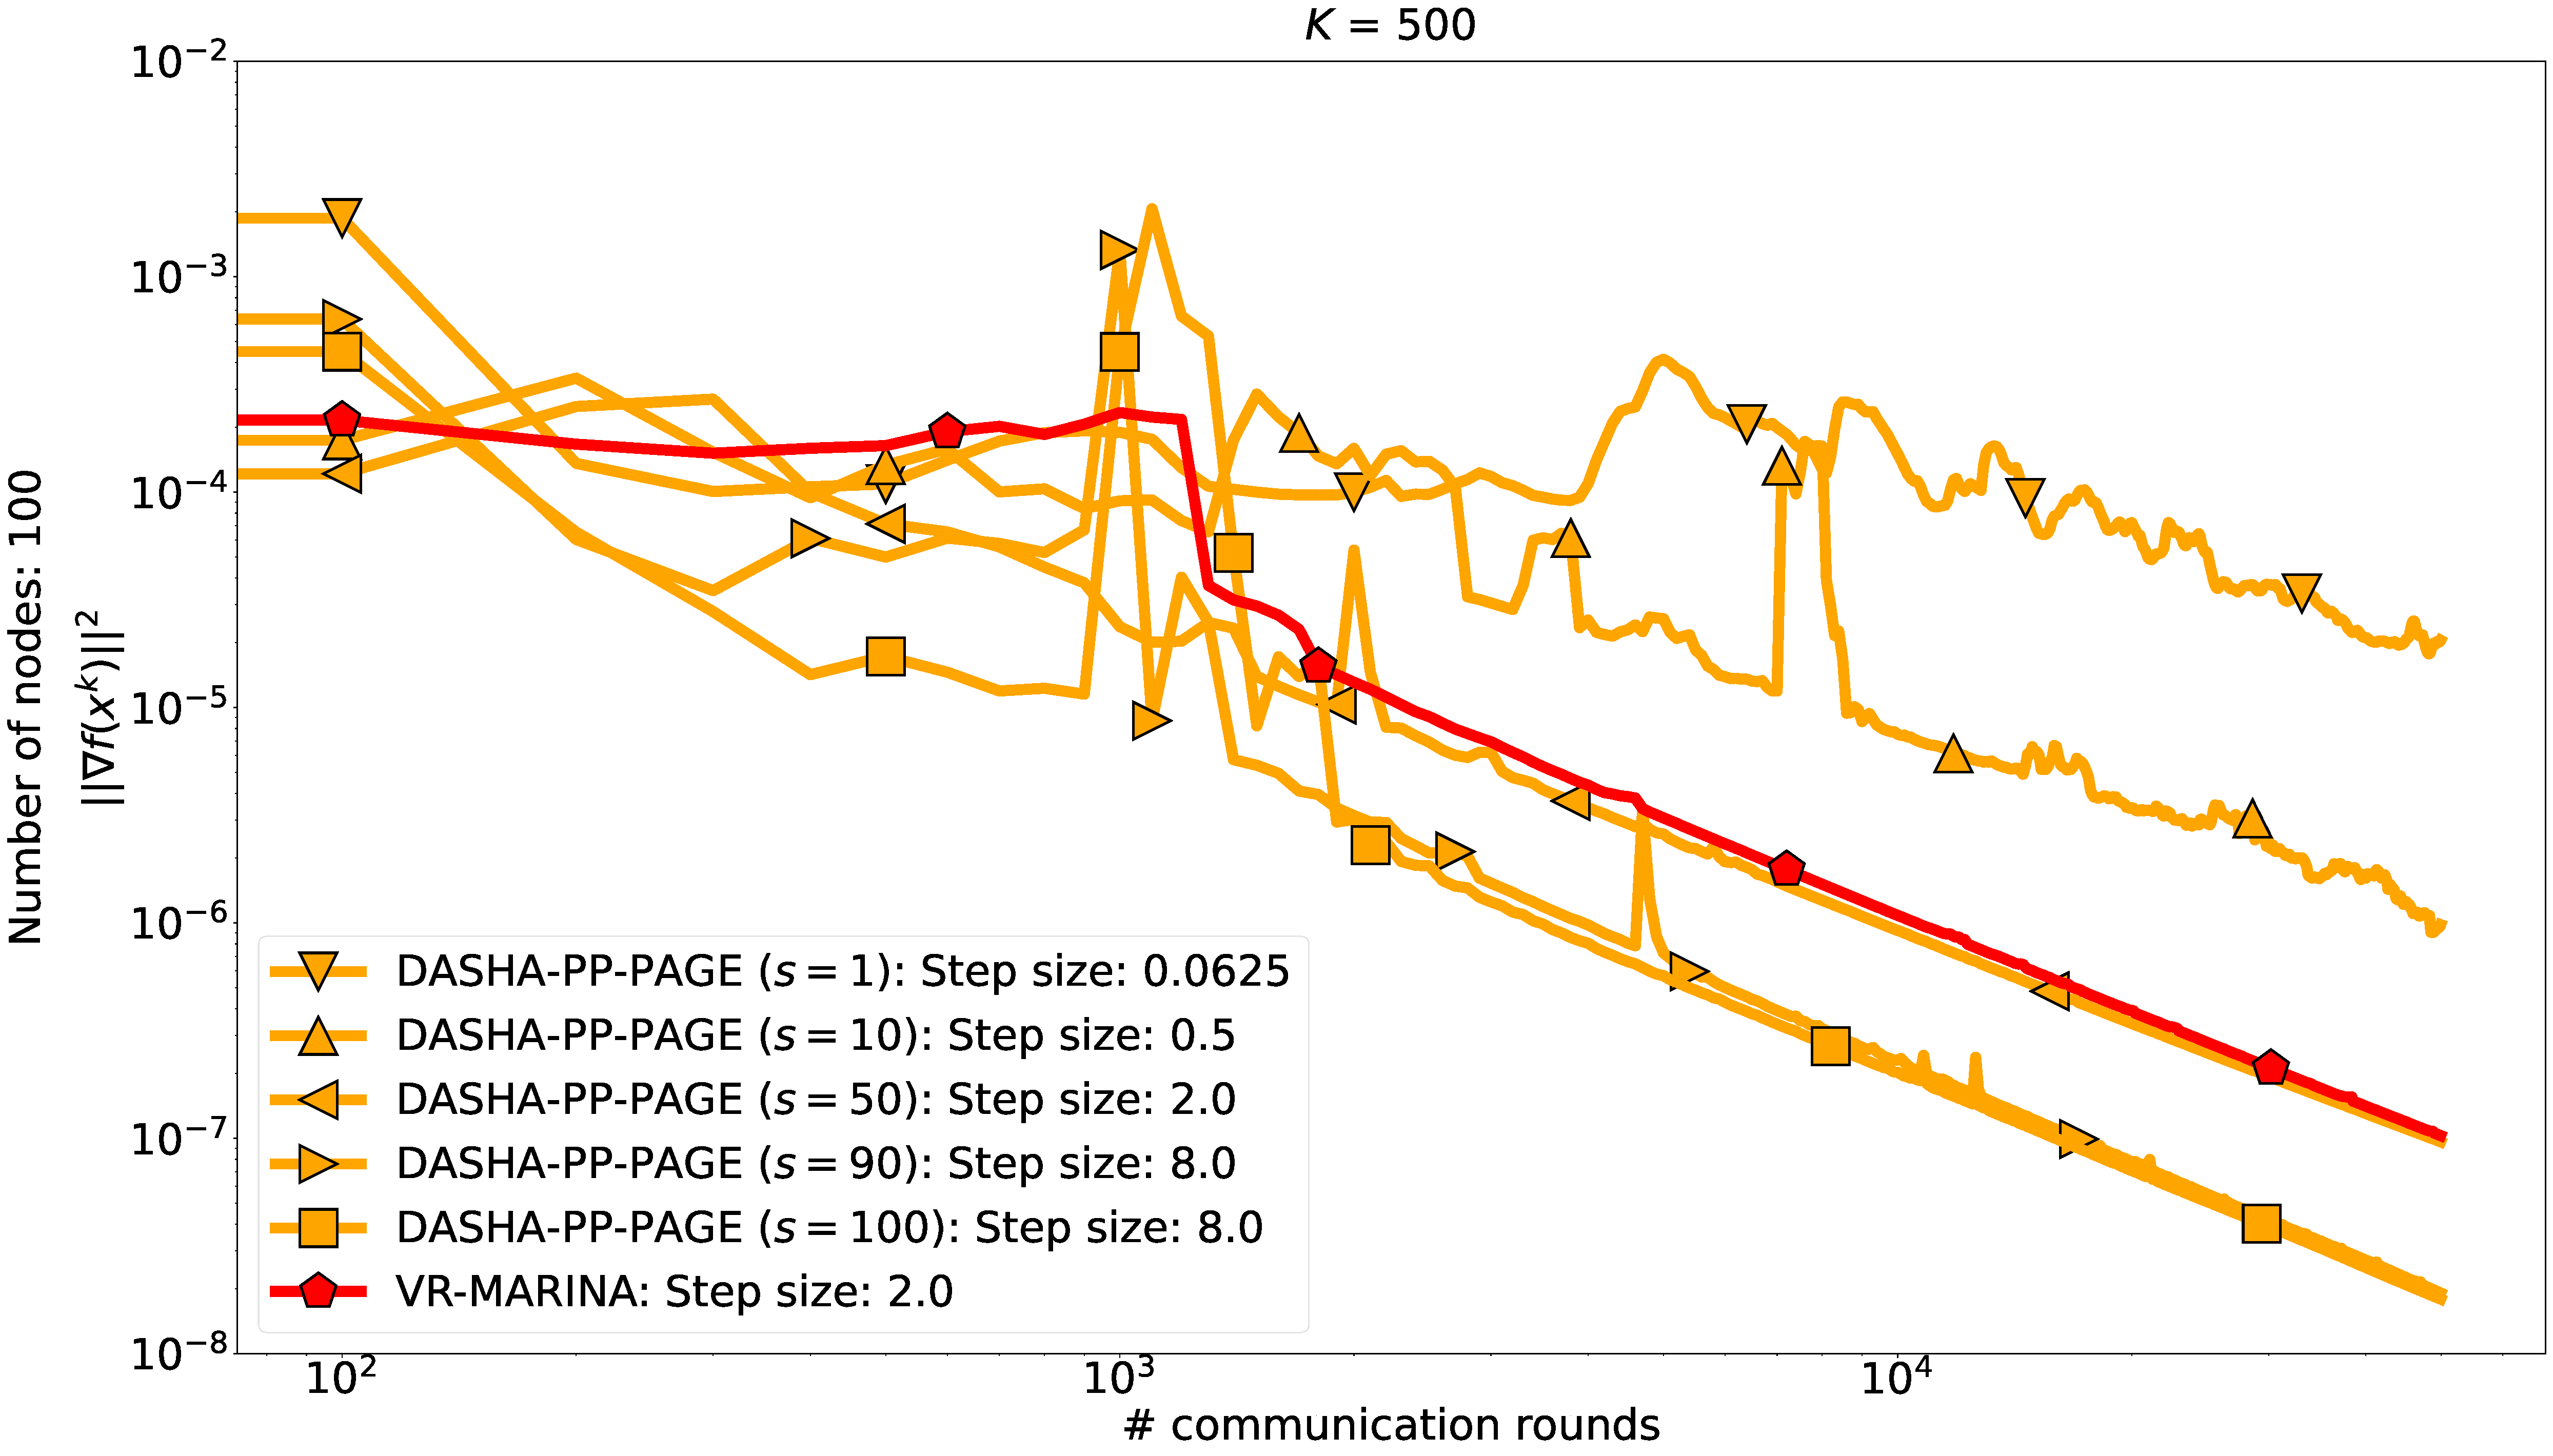
\includegraphics[width=\textwidth]{neurips_2022_finite_sum_real-sim_nof_500_numnodes_100_more_probs_batch_size_1.pdf}
%         \caption{REAL-SIM, BZ = 1}
%     \end{subfigure}
%     \begin{subfigure}{.5\textwidth}
%         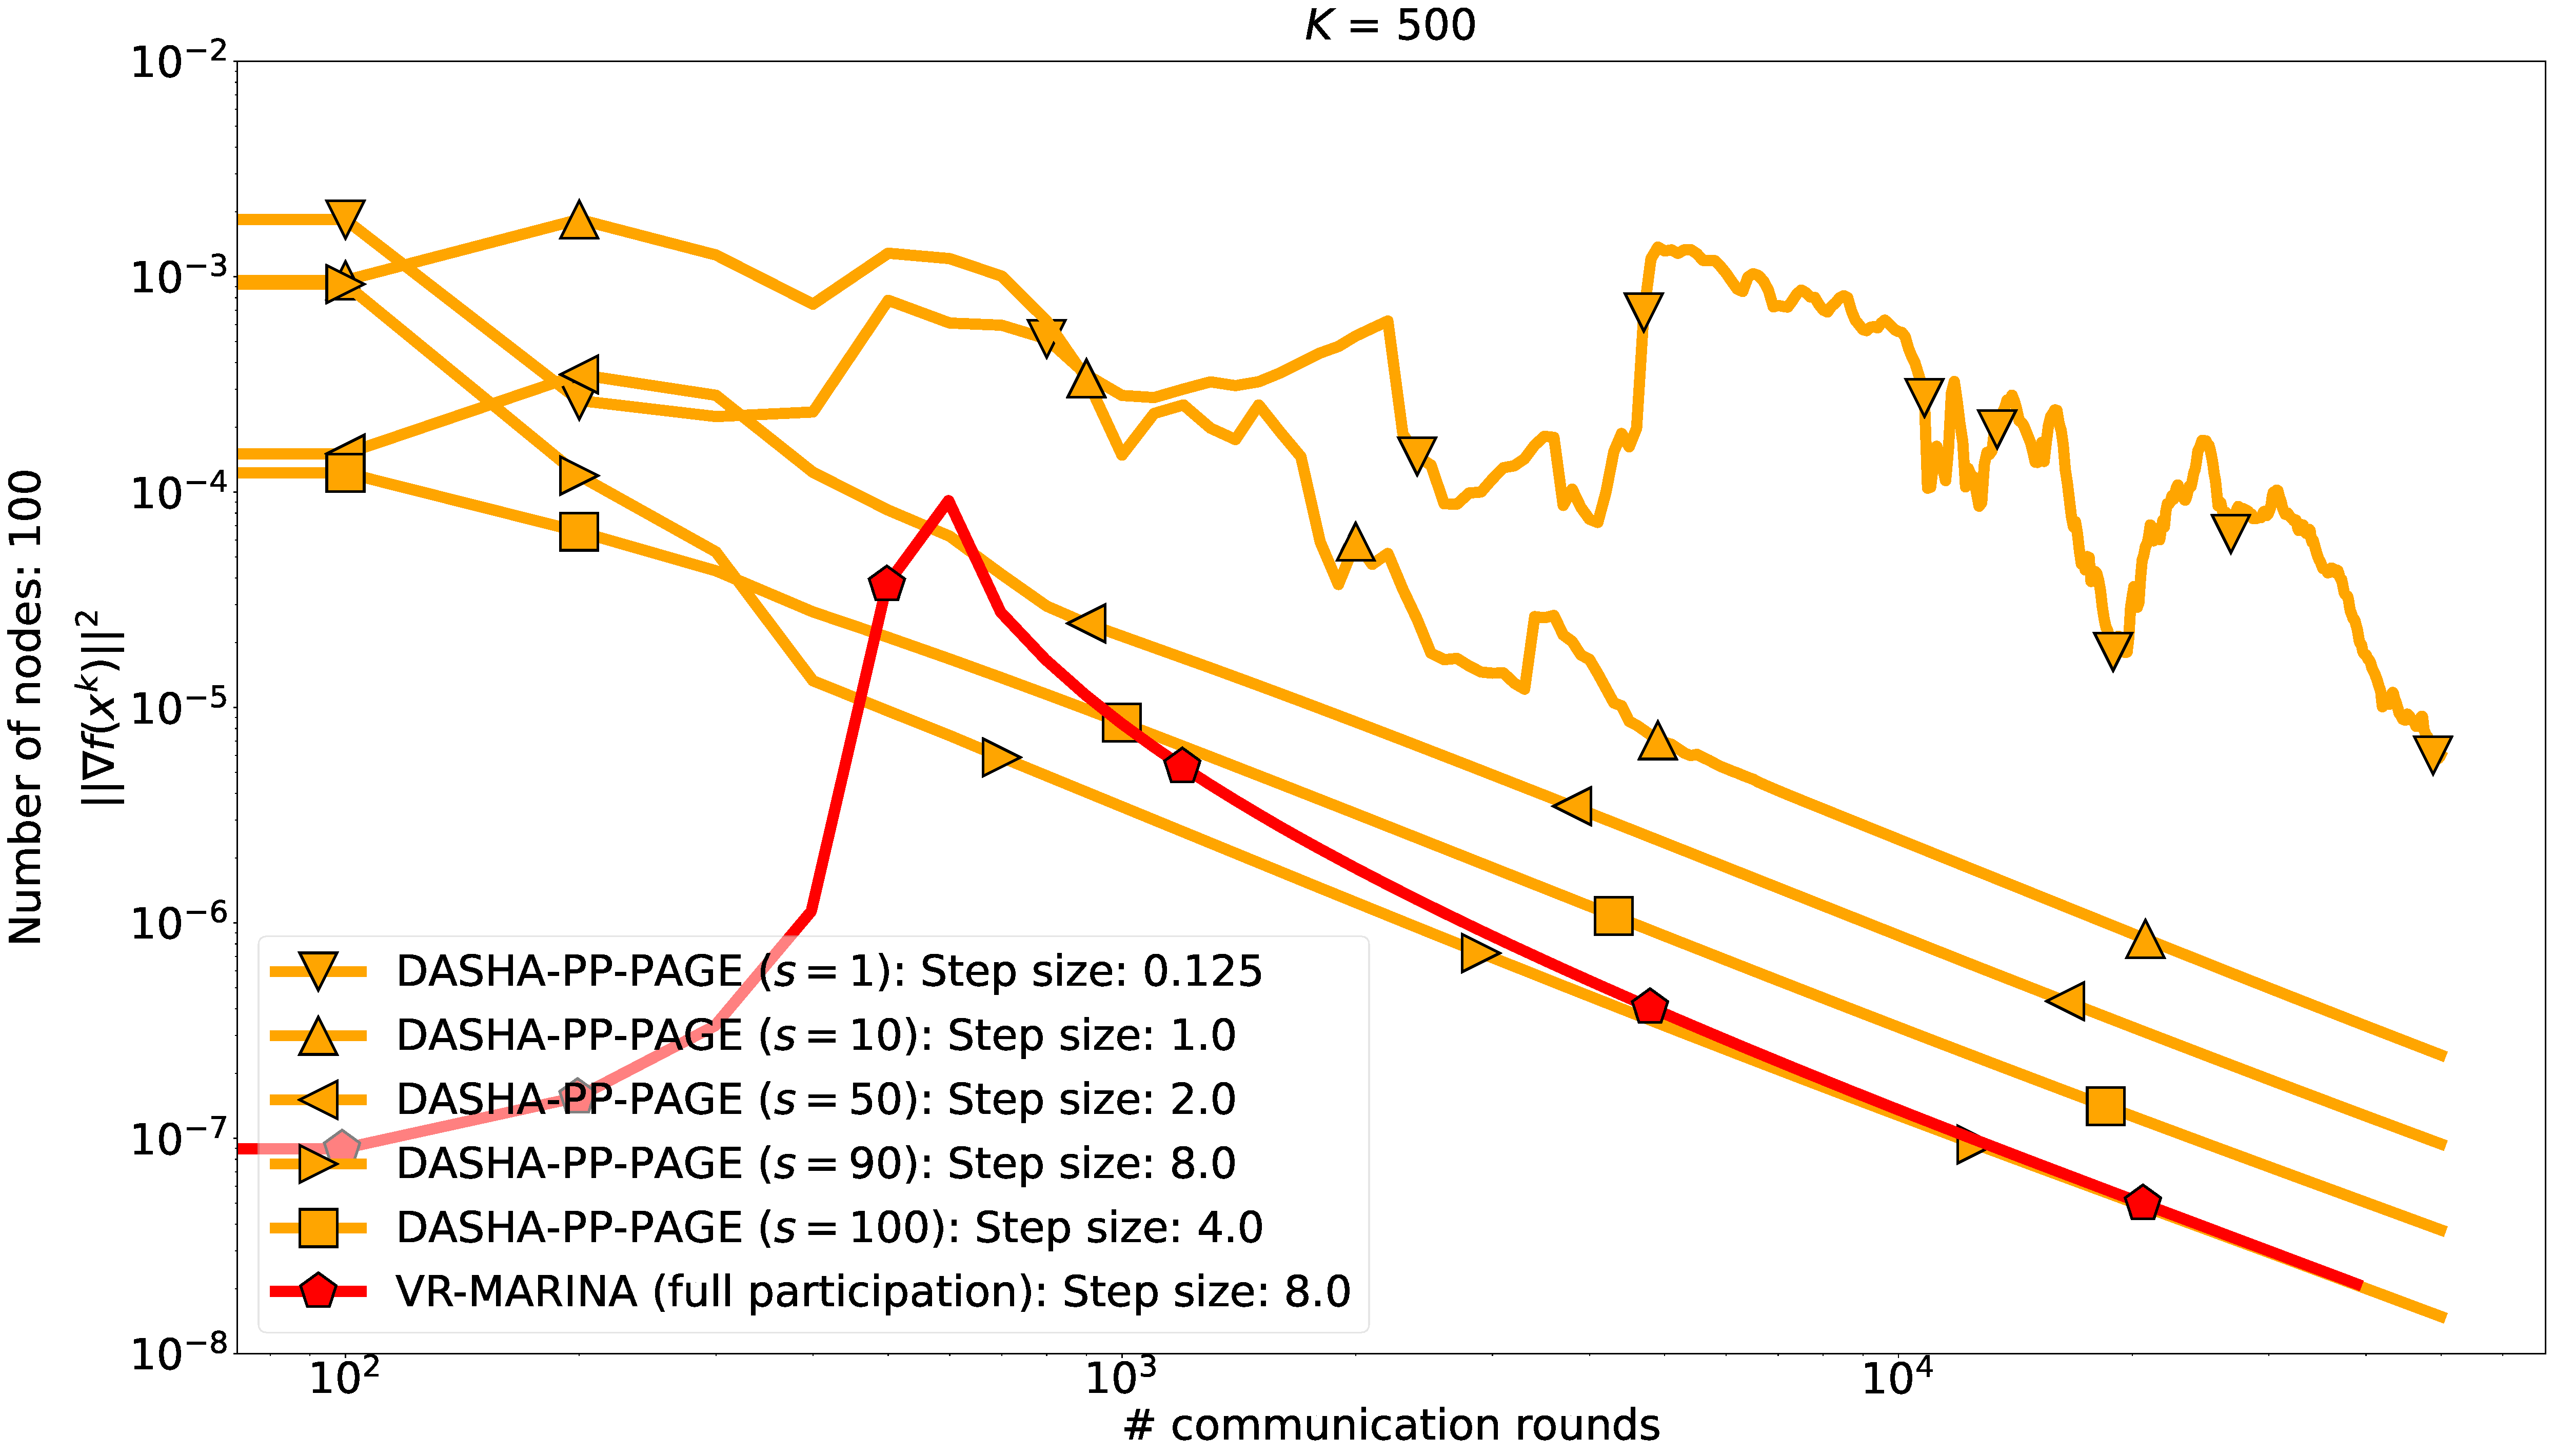
\includegraphics[width=\textwidth]{neurips_2022_finite_sum_real-sim_nof_500_numnodes_100_more_probs_batch_size_1000.pdf}
%         \caption{REAL-SIM, BZ = 1000}
%     \end{subfigure}
% \caption{Classification task with the \textit{mushrooms} dataset.}
% \label{fig:finite-sum-real-sim}
% \end{figure}

\end{document}
